\chapter{Objetivo}

O objetivo do trabalho é discutir as principais técnicas para reconhecimento de gestos e poses de mão em um ambiente automotivo.
Os algoritmos e metodologias hoje utilizados para segmentar e extrair características de imagens e vídeos devem ser estudados e verificados se atingem seu propósito em um ambiente automotivo. Esse ambiente apresenta uma forte variação de luz e ausência de controle nas características da mão e do braço do motorista (cor de pele, braço com ou sem vestimentas e vestimentas de cores e estampas diferentes). As características extraídas são utilizadas como entrada em um classificador responsável por reconhecer gestos e poses de mão, e assim, permitir uma interação com o veículo traduzindo os gestos em comandos para o carro.

Reconhecimento de gestos baseado em visão é um assunto bastante popular e pesquisado. A busca por mecanismos que tornem a interação entre homem e máquina mais intuitiva e natural é constante e vem aumentando com o lançamento de plataformas que auxiliam os desenvolvedores nos complexos algoritmos que envolvem essa área.
O lançamento do Kinect, da Microsoft \cite{kinect}, e da plataforma de desenvolvimento da Intel, chamada Intel Perceptual Computing \cite{intel} (ambas com câmeras de profundidade) vem popularizando o desenvolvimento de aplicativos e revolucionando o jeito que interagimos com os jogos e computadores. 

\begin{figure}[ht!]
\centering
\fbox{
  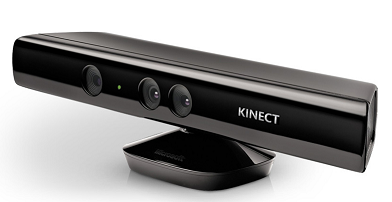
\includegraphics[width=0.3\textwidth]{image/kinect_camera.png}
  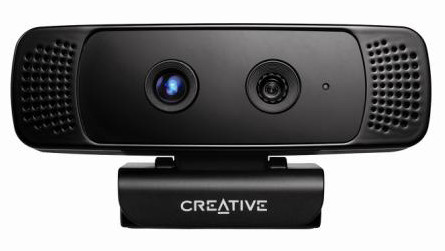
\includegraphics[width=0.3\textwidth]{image/intel_creative_camera.jpg}}
  \caption{Kinect, da Microsoft, e a câmera da \textit{Creative} com parceria da Intel}
  \label{fig:depth_camera}
\end{figure}

O uso de câmeras em carros e caminhões também tem aumentando nos últimos anos. Sistemas de segurança capazes de verificar se o motorista esta saindo indevidamente da faixa, ou se o veículo esta em rota de colisão com algum outro automóvel ou objeto e até mesmo monitorando o stress do motorista já são comuns em vários modelos de veículos. Mas pouco vimos o uso dessas câmeras para interação do motorista com a grande quantidade de controles que temos no carro. Aumentar ou diminuir o volume do rádio, trocar de faixa de música, dar zoom no mapa do sistema de navegação são alguns exemplos de comandos que poderia ser dados através de gestos.
O sistema de gestos também pode ser usado como um complemento ao sistema de reconhecimento de voz, bastante comum hoje nos carros e que funciona muito bem.

As condições gerais dentro do automóvel inclui uma grande variação de iluminação, mudança de usuário e fundos não uniformes. Além disso, a aceitação do usuário é um item bastante importante, portanto coisas como uma iluminação artificial visível, restrição de vestimentas e calibração extensiva não pode ser tolerado. Tento isso em mente, alguns critérios e requisitos para o sistema podem ser estabelecidos:

\begin{itemize}
\item robustez contra ambientes ruidosos
\item iluminação invisível
\item independente de usuário
\item sem calibração ou treinamento pelo usuário
\item pequeno e compreensível conjunto de gestos
\item reação do sistema com o mínimo de latência
\end{itemize}


